\paragraph{UC1.1.2 - Caricamento dal database}

\mbox{}

\begin{figure}[h]
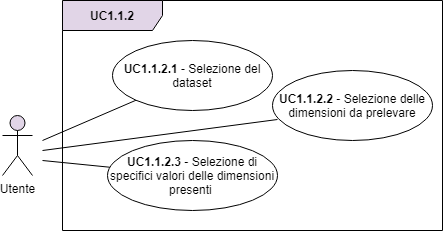
\includegraphics[width=12cm]{section/Images/UC1.1.2.png}
\centering
\caption{UC1.1.2 - Caricamento dati da database}
\end{figure}

\begin{itemize}
	\item \textbf{Attore primario}: Utente;
	\item \textbf{Precondizioni}: Il sistema è raggiungibile e funzionante. Il database contiene almeno un dataset;
	\item \textbf{Postcondizioni}: I dati e le dimensioni vengono caricati nel sistema. Viene visualizzato un messaggio che avvisa l'utente del corretto caricamento e della loro validità;
	\item \textbf{Scenario principale}: 
	\begin{enumerate}
			\item Viene presentata all'utente una lista con i dataset presenti nel database;
			\item L'utente seleziona uno tra i dataset disponibili [UC1.1.2.1];
			\item L'utente seleziona le dimensioni dal dataset scelto [UC1.1.2.2];
			\item L'utente, eventualmente, seleziona specifici valori dalle dimensioni scelte [UC1.1.2.3];
			\item L'utente preme un pulsante per confermare la scelta e salvare i dati nel sistema.
		\end{enumerate}
	
\end{itemize}

\subparagraph{UC1.1.2.1 - Selezione del dataset}
\begin{itemize}
	\item \textbf{Attore primario}: Utente;
	\item \textbf{Precondizioni}: Il sistema è raggiungibile e funzionante. Il database contiene almeno un dataset;
	\item \textbf{Postcondizioni}: Il dataset da prelevare viene selezionato;
	\item \textbf{Scenario principale}: L'utente seleziona uno dei dataset tra quelli disponibili all'interno del database.
	
\end{itemize}

\subparagraph{UC1.1.2.2 - Selezione delle dimensioni da prelevare}
\begin{itemize}
	\item \textbf{Attore primario}: Utente;
	\item \textbf{Precondizioni}: Il sistema è raggiungibile e funzionante. Il database contiene almeno un dataset;
	\item \textbf{Postcondizioni}: Le dimensioni da prelevare vengono selezionate;
	\item \textbf{Scenario principale}: L'utente seleziona le dimensioni che vuole importare dal database tra quelle presenti nel dataset.
	
\end{itemize}

\subparagraph{UC1.1.2.3 - Selezione di specifici valori delle dimensioni presenti}
\begin{itemize}
	\item \textbf{Attore primario}: Utente;
	\item \textbf{Precondizioni}: Il sistema è raggiungibile e funzionante. Il database contiene almeno un dataset;
	\item \textbf{Postcondizioni}: I dati da prelevare vengono selezionati;
	\item \textbf{Scenario principale}: L'utente seleziona i dati che vuole importare dal database ponendo specifiche condizioni alla query di selezione.
	
\end{itemize}